\documentclass[pdftex,fleqn,a4paper]{article}
  
  \let\oldAuthor\author
  \renewcommand{\author}[1]{\newcommand{\theAuthor}{#1}\oldAuthor{#1}} 
  \let\oldTitle\title
  \renewcommand{\title}[1]{\newcommand{\theTitle}{#1}\oldTitle{#1}}
  \newcommand{\subtitle}[1]{\newcommand{\theSubtitle}{#1}}
  \let\oldDate\date
  \renewcommand{\date}[1]{\newcommand{\theDate}{#1}\oldDate{#1}}
  
  \usepackage{../huisstijl/vubtitlepage}
  \faculty{Faculteit Ingenieurswetenschappen}
  
  \author{\href{mailto:Egon.Geerardyn@vub.ac.be}{Egon Geerardyn}}
  \title{Formules Chemie}
  \newcommand{\revisie}{revisie 0.4b}
  \date{\revisie\ (\today)}
 
 
 
 
  %\usepackage{graphicx}
  \usepackage{amsfonts}
  \usepackage{mathrsfs}
  \usepackage{fancyhdr}
  \usepackage[dutch]{babel}
  \usepackage[latin1]{inputenc}
  \usepackage[T1]{fontenc}
  \usepackage[pdftex]{hyperref}
  \usepackage{flow}
  \usepackage{graphicx}
  \usepackage{wrapfig}
  \usepackage{rotating}
  %%%%

  \addtolength{\textheight}{2cm}
  \addtolength{\textwidth}{3cm}
  \addtolength{\hoffset}{-1.5cm}
  \renewcommand{\rmdefault}{cmss}
  \renewcommand{\sfdefault}{cmr}


     % Egon Geerardyn common latex Commands
%
% 2007 01 03 : Version 0.5
%
%
%
% dependencies
\usepackage[usenames]{color}
\usepackage{amsfonts}
\usepackage{mathrsfs}
% hyperlinks (pdfLaTeX)
    \newcommand{\tildefix}{\textasciitilde}
    \newcommand{\hreftt}[2]{\href{#1}{\texttt{#2}}} %teletype set link
    \newcommand{\link}[1]{\href{#1}{#1}}
    \newcommand{\linktt}[1]{\hreftt{#1}{#1}}


% symbolen
  %   \usepackage{manfnt}
  % \newcommand{\vb}{\mbox{\manstar}}
   \newcommand{\qed}{\mbox{$\Box$}}
   \newcommand{\QED}{\begin{flushright}\qed\end{flushright}}
   \newcommand{\GO}{\mbox{$\{\aleph\}$}}
   \newcommand{\n}{\mbox{$^{\mbox{n}}$}}
   \newcommand{\e}{\mbox{$^{\mbox{e}}$}}
   \newcommand{\s}{\mbox{$^{\mbox{s}}$}}
     \usepackage{wasysym}
   \newcommand{\ctr}{\mbox{\lightning}}
   \newcommand{\cte}{\mathrm{ct{^{\underline{\mathrm{e}}}}}}
   \newcommand{\vgl}{\mbox{vgl}}
   \newcommand{\hn}{\mbox{$\overline{\mbox{h}}$}}
   \newcommand{\wn}{\mbox{$\overline{\mbox{w}}$}}
   \newcommand{\zn}{\mbox{$\overline{\mbox{z}}$}}
   \newcommand{\RA}{\mbox{$\Longrightarrow$}}
   \newcommand{\LA}{\mbox{$\Longleftarrow$}}
   \newcommand{\LRA}{\mbox{$\Longleftrightarrow$}}
   \newcommand{\rer}{\mbox{$\sim$}}
   \newcommand{\isdef}{\mbox{$\stackrel{\Delta}{=}$}}
   \newcommand{\elek}{\mbox{$e^{-}$}}
   \newcommand{\prot}{\mbox{$p^{+}$}}
   \newcommand{\neut}{\mbox{$n^{0}$}}
   \newcommand{\angstrom}{\eenh{\AA}}
     \let\SavedRightarrow=\Rightarrow %fix for Marvosym rightarrow
       \usepackage{marvosym}
     \let\Rightarrow=\SavedRightarrow %fix for Marvosym rightarrow
   \newcommand{\wwwsym}{\Ecommerce}
   \newcommand{\www}[1]{\wwwsym\ #1}
   \newcommand{\pompern}{\mbox{\Gentsroom}}
   \newcommand{\busbitch}{\Ladiesroom}
   \newcommand{\msun}{m_{\odot}}
   \newcommand{\mearth}{m_{\earth}}
   \newcommand{\rearth}{r_{\earth}}
   \newcommand{\GOis}{\stackrel{$\GO$}{\approx}}

%invultemplates
   \newcommand{\invulW}{\qquad \qquad \qquad \quad}
   \newcommand{\invulWs}{\qquad \qquad \qquad}
   \newcommand{\invulF}{\pm \qquad \qquad \quad}
   \newcommand{\invulM}{\qquad \quad}
   \newcommand{\invulWF}{\invulW \invulF}
   \newcommand{\invulWFM}{\left(\invulWF\right) \cdot \invulM}
   \newcommand{\invulT}[1]{\vspace{#1}}
   \newcommand{\foutenentry}[2]{ #1      & $\invulW$ & $#2$ \\ \hline}
   \newcommand{\tablesizer}[1]{\renewcommand\arraystretch{#1}}
   \newcommand{\bigtables}{\tablesizer{2.0}}
   \newcommand{\normtables}{\tablesizer{1.0}}
   \newcommand{\foutenbespreking}[2]{\bigtables
                                      \begin{tabular}{|l|rl|}
                                          \hline
                                        \foutenentry{\textbf{Waarde} $#2$}{#1}
                                          \hline
                                        \foutenentry{Afleesfout}{#1}
                                        \foutenentry{Instelfout}{#1}
                                        \foutenentry{Instrumentfout}{#1}
                                        \foutenentry{Nulpuntsfout}{#1}
                                          \hline
                                        \foutenentry{\textbf{Totale absolute fout}}{#1}
                                          \hline
                                        \foutenentry{\textbf{Totale relatieve fout}}{}
                                      \end{tabular}
                                     \normtables
                                    }
   \newcommand{\foutenbesprekingkort}[2]{\bigtables
                                      \begin{tabular}{|l|rl|}
                                          \hline
                                        \foutenentry{\textbf{Waarde} $#2$}{#1}
                                          \hline
                                        \foutenentry{\textbf{Totale relatieve fout}}{}
                                        \foutenentry{\textbf{Totale absolute fout}}{#1}
                                      \end{tabular}
                                     \normtables
                                    }

% dutch arc-goniometric functions
    \newcommand{\bgsin}{\mbox{\textsf{Bgsin}}\,}
    \newcommand{\bgcos}{\mbox{\textsf{Bgcos}}\,}
    \newcommand{\bgtan}{\mbox{\textsf{Bgtan}}\,}
    \newcommand{\bgcot}{\mbox{\textsf{Bgcot}}\,}

%alternative notation for arc-goniometric functions
    \newcommand{\argcos}{\mbox{\textsf{argcos}}\,}
    \newcommand{\argsin}{\mbox{\textsf{argsin}}\,}
    \newcommand{\argtan}{\mbox{\textsf{argtan}}\,}
    \newcommand{\argcot}{\mbox{\textsf{argcot}}\,}

%alternative notation for arc-hyperbolic functions
    \newcommand{\argcosh}{\mbox{\textsf{argcosh}}\,}
    \newcommand{\argsinh}{\mbox{\textsf{argsinh}}\,}
    \newcommand{\argtanh}{\mbox{\textsf{argtanh}}\,}
    \newcommand{\argcoth}{\mbox{\textsf{argcoth}}\,}

% coordinaat
    \newcommand{\co}{\mbox{ \textsf{co}}\,}
% absolute waarde
    \newcommand{\abs}[1]{\left| #1 \right|}
% degree symbol
    \newcommand{\degree}[0]{^\circ}
    \newcommand{\degC}[0]{\; \degree \eenh{C}}
% ronde B voor bol
    \newcommand{\bol}[0]{\mathscr{B}}

% ronde K voor kwadriek
    \newcommand{\kwadriek}[0]{\mathscr{K}}

%differentials
    \renewcommand{\d}[1]{\;\textsf{d}#1}
    \newcommand{\pd}[1]{\partial #1}
    \newcommand{\D}{\;\textsf{D}}
    \newcommand{\pdiff}[3][]{\frac{\pd^{#1}{#2}}{\pd{#3}^{#1}}}
    \newcommand{\diff}[3][]{\frac{\d^{#1}{#2}}{\d{#3}^{#1}}}

%dot and double dot for D_t en D_t^2
    \newcommand{\dt}[1]{\dot{#1}} %dot notation for d/dt
    \newcommand{\dtt}[1]{\ddot{#1}} % double dot notation for d^2 / dt^2

%accent (acute) for D_s and D_s^2
    \newcommand{\ds}[1]{#1 \acute{}\,} % accent notation for d/ds
    \newcommand{\dss}[1]{#1 \acute{}\, \acute{}\,} % double accent notation for d^2 / ds^2

%accent notation for arbitrrary derivative of order 1 or 2
    \newcommand{\dx}[1]{#1 \grave{}\,} % accent notation for arbitrary d / dx
    \newcommand{\dxx}[1]{#1 \grave{} \, \grave{}\,} % double accent notation for d^2 / dx^2

%differential operators
    \newcommand{\vnabla}{\vec{\nabla}}
    \newcommand{\Nabla}{\vnabla}
    % nabla notated
    \newcommand{\vgradN}[1]{\Nabla #1\;}
    \newcommand{\vrotN}[1]{\Nabla \times #1\;}
    \newcommand{\vdivN}[1]{\Nabla \cdot #1\;}
    % standard (Dutch) notated
    \newcommand{\vgradT}[1]{\;\vec{\textsf{grad}}\,#1\;}
    \newcommand{\vrotT}[1]{\;\vec{\textsf{rot}}\,#1\;}
    \newcommand{\vdivT}[1]{\;\textsf{div}\,#1\;}
    % wrapper for easy switching
    \newcommand{\vgrad}[1]{\vgradT{#1}}
    \newcommand{\vrot}[1]{\vrotT{#1}}
    \newcommand{\vdiv}[1]{\vdivT{#1}}

%norm of a vector
    \newcommand{\norm}[1]{\left\| #1 \right\|}

%infinity redeclariation for use with WikiPedia LaTeX notation
    \newcommand{\infin}{\infty}

%Probability notation
    \newcommand{\prob}[1]{P\left(#1\right)}

%Combination
    \newcommand{\combination}[2]{\left( \begin{array}{c} #1 \\ #2 \end{array} \right)}

% E and Var
    \newcommand{\E}[1]{\!\mathrm{E}\left[ #1 \right]}
    \newcommand{\Var}[1]{\!\mathrm{Var}\left[ #1 \right]}

%identieke matrix
    \newcommand{\idmatrix}{\textsf{I}}
    \newcommand{\spoor}[1]{\mbox{\textsf{sp}}\left( #1 \right)\,}
%signumfunctie
    \newcommand{\sign}[1]{\textsf{sign}\left( #1 \right)}
%regel van de l'hopital
    \newcommand{\hopital}{\stackrel{\textsf{H}}{=}}
%vector functions
    % vector notation
    \newcommand{\vect}[1]{\overline{#1}} %large notation
    %(scalar product, <>-notation
    \newcommand{\scalprod}[2]{\left\langle #1,#2 \right\rangle}
    \newcommand{\scalprodv}[2]{\scalprod{\vec{#1}}{\vec{#2}}} %includes vector arrows
    \newcommand{\scalprodV}[2]{\scalprod{\vect{#1}}{\vect{#2}}}
    %vectorr product
    \newcommand{\vectprod}[2]{\left( #1 \times #2 \right)}
    \newcommand{\vectprodv}[2]{\vectprod{\vec{#1}}{\vec{#2}}} % includes vector arrows
    \newcommand{\vectprodV}[2]{\vectprod{\vect{#1}}{\vect{#2}}}
    %gradient, rotatie, divergentie
    \newcommand{\Dgrad}[1]{\textsf{grad}\,#1\;}
    \newcommand{\Ddiv}[1]{\textsf{div}\,#1\;}
    \newcommand{\Drot}[1]{\textsf{rot}\,#1\;}

%chemistry
    %concentration
    \newcommand{\conc}[1]{\left[ #1 \right]}
    %equilibrum arrows
    \newcommand{\evenwicht}{\rightleftharpoons}
    \newcommand{\reactie}{\rightarrow}
    %reactieconstante
    \newcommand{\K}{\,\textsf{K}}
    \newcommand{\Q}{\,\textsf{Q}}
    %p-notations
    \newcommand{\pH}{\,\textsf{pH}}
    \newcommand{\pOH}{\,\textsf{pOH}}
    \newcommand{\pK}{\,\textsf{pK}}
    \newcommand{\pKa}{\pK_A}
    \newcommand{\pKb}{\pK_B}
    \newcommand{\pKw}{\pK_W}
    %eenheden
    \newcommand{\eenheid}[1]{\,\textsf{#1}\,}
    \newcommand{\eenh}[1]{\eenheid{#1}}
    \newcommand{\Vr}{\,\textsf{Vr}\,}
    \newcommand{\molaliteit}{\mathbf{m}}
    \newcommand{\molar}[1]{\overline{#1}}
    \newcommand{\standard}[1]{#1^{\circ}}

% tango colors
   \definecolor{TangoButter1}{rgb}{0.9882, 0.9137, 0.3098}
   \definecolor{TangoButter2}{rgb}{0.9294, 0.8313, 0.0000}
   \definecolor{TangoButter3}{rgb}{0.7686, 0.6274, 0.0000}

   \definecolor{TangoOrange1}{rgb}{0.9882, 0.6863, 0.2431}
   \definecolor{TangoOrange2}{rgb}{0.9608, 0.4745, 0.0000}
   \definecolor{TangoOrange3}{rgb}{0.8078, 0.3608, 0.0000}

   \definecolor{TangoChocolate1}{rgb}{0.9137, 0.7255, 0.4314}
   \definecolor{TangoChocolate2}{rgb}{0.7569, 0.4902, 0.0667}
   \definecolor{TangoChocolate3}{rgb}{0.5608, 0.3490, 0.0078}

   \definecolor{TangoChameleon1}{rgb}{0.5412, 0.8863, 0.2039}
   \definecolor{TangoChameleon2}{rgb}{0.4510, 0.8235, 0.0863}
   \definecolor{TangoChameleon3}{rgb}{0.3059, 0.6039, 0.0235}

   \definecolor{TangoSkyBlue1}{rgb}{0.4471, 0.6235, 0.8118}
   \definecolor{TangoSkyBlue2}{rgb}{0.2039, 0.3961, 0.6431}
   \definecolor{TangoSkyBlue3}{rgb}{0.1255, 0.2902, 0.5294}

   \definecolor{TangoPlum1}{rgb}{0.6784, 0.4980, 0.6588}
   \definecolor{TangoPlum2}{rgb}{0.4588, 0.3137, 0.4824}
   \definecolor{TangoPlum3}{rgb}{0.3608, 0.2078, 0.4000}

   \definecolor{TangoScarletRed1}{rgb}{0.9373, 0.1608, 0.1608}
   \definecolor{TangoScarletRed2}{rgb}{0.8000, 0.0000, 0.0000}
   \definecolor{TangoScarletRed3}{rgb}{0.6431, 0.0000, 0.0000}

   \definecolor{TangoScarletRed1}{rgb}{0.9373, 0.1608, 0.1608}
   \definecolor{TangoScarletRed2}{rgb}{0.8000, 0.0000, 0.0000}
   \definecolor{TangoScarletRed3}{rgb}{0.6431, 0.0000, 0.0000}

   \definecolor{TangoAluminium1}{rgb}{0.9333, 0.9333, 0.9255}
   \definecolor{TangoAluminium2}{rgb}{0.8275, 0.8431, 0.8118}
   \definecolor{TangoAluminium3}{rgb}{0.7294, 0.7412, 0.8392}
   \definecolor{TangoAluminium4}{rgb}{0.5333, 0.5412, 0.5216}
   \definecolor{TangoAluminium5}{rgb}{0.3333, 0.3412, 0.3255}
   \definecolor{TangoAluminium6}{rgb}{0.1804, 0.2039, 0.2118}

% opmaak
    \newcommand{\opmerking}{\par\textbf{\color{TangoScarletRed3}{Opmerking: }}}
    \newcommand{\pro}{$\Box\!\!\!\!$\color{TangoChameleon3}{\ding{52}}}
    \newcommand{\con}{$\Box\!\!\!\!$\color{TangoScarletRed2}{\ding{56}}$\;$}
    \newcommand{\warn}{$\Box\!\!\!\!\!$\color{TangoSkyBlue2}{\ding{72}}$\;$}

% average over time
    \newcommand{\average}[1]{\left\langle #1\right\rangle}


    \newcommand{\definitie}[2]{\par \textbf{#1:}  #2\par}

  
 %lay-out
  \hypersetup{colorlinks,%
            citecolor=black,%
            filecolor=black,%
            linkcolor=black,%
            urlcolor=black,%
            pdfauthor={Egon Geerardyn},%
            pdftitle={Formules Chemie},%
            plainpages=false}%,%
            %pdfpagelabels}
  \pdfpagewidth=\paperwidth
  \pdfpageheight=\paperheight
 %margins
\begin{document}
  \maketitlepage
%  \titlepage
%  \thispagestyle{empty}%
%  \null
%  \vfill
%  \begin{center}\leavevmode
%    \normalfont
%    %{\Large\raggedleft schooljaren 2004 -- 2005 -- 2006\par}%
%    {\Large\raggedleft Ingenieurswetenschappen\par}%
%    \hrulefill\par
%    {\Huge\raggedright Formularium Chemie \large \revisie\   \footnotesize (\today)\par }%
%  \end{center}%
%  \vfill
%  \footnotesize
%  auteur: \textsc{E. Geerardyn}\par
%  bron: \textsc{prof. R. Willem}, \textit{Chemie: Structuur en Transformaties van de materie}, Dienst Uitgaven VUB 2006.\par
%  bron: \textsc{prof. M. Biesemans} en \textsc{prof. R. Willem} , \textit{Chemie: Oefeningen}, Dienst Uitgaven VUB 2006.\par
%  bron: \textsc{Brown, LeMay} en \textsc{Bursten} , \textit{Chemistry: the Central Science (10th Edition)}, Pearson Education 2006.
%  \normalsize
%  
%  \null
    \setlength{\voffset}{-2cm}
  
  \newpage

  \pagestyle{fancy}
  \rhead{pagina \thepage}
  \chead{\footnotesize \revisie}
  \lhead{\textbf{Formules Chemie}}
  \cfoot{}
   \section*{Voorwoord}
\label{sec:Voorwoord}
  Deze uitgave is geen officiële uitgave van de Vrije Universiteit Brussel, slechts een formularium gemaakt door een student.
  Mogelijk staan er hier of daar nog fouten in, indien u er tegenkomt,
  stuur gerust een mailtje naar \hreftt{mailto:egon.geerardyn@vub.ac.be}{egon.geerardyn@vub.ac.be}.\par

  \begin{quote}
    Copyright \copyright{}  Egon Geerardyn.\par
    Permission is granted to copy, distribute and/or modify this document
    under the terms of the GNU Free Documentation License, Version 1.2
    or any later version published by the Free Software Foundation;
    with no Invariant Sections, no Front-Cover Texts, and no Back-Cover Texts.
    A copy of the license is included in the section entitled ``GNU
    Free Documentation License'' in the source code and available on:
    \linktt{http://www.gnu.org/copyleft/fdl.html}.
  \end{quote}
  \noindent
  De \LaTeX -broncode is vrij beschikbaar onder GNU Free Document License. \par


  Mogelijk is er reeds een nieuwe versie beschikbaar op\par
  \hreftt{http://students.vub.ac.be/~egeerard/projects.html}{http://students.vub.ac.be/\tildefix egeerard/projects.html}
\section*{Referenties}
\begin{enumerate}
	\item \textsc{D. Lefeber}, \textit{Mechanica: Deel I}, Dienst Uitgaven VUB 2006.
	\item \textsc{D. Lefeber}, \textit{Mechanica: Deel II}, Dienst Uitgaven VUB 2006.
        \item \textsc{D. Lefeber}, \textit{Mechanica met ontwerpproject}, Polytechnische Kring 2007.
        \item \textsc{D. Van Hemelrijck}, \textit{Mechanica van materialen, mechanismen en vloeistoffen}, Pointcarré 2008.
	\item \textsc{D. Vandepitte}, \linktt{http://www.berekeningvanconstructies.be}, 2006.
\end{enumerate}



   \newpage
   \tableofcontents
   \newpage
   
  % \newpage
\section{Gaswetten}
\label{sec:Gaswetten}


  % \newpage
\section{Stoichiometrie}
\label{sec:Stoichiometrie}


   
   \onecolumn
\newpage
\section{Chemische Thermodynamica}
\label{sec:H:Thermodynamica}

\paragraph{Tekenconventie} voor energie-overdracht
\label{sec:Tekenconventie}
\[
  \mbox{systeem} \stackrel{-}{\rightarrow} \mbox{buitenwereld}
\]
\[
  \mbox{systeem} \stackrel{+}{\leftarrow} \mbox{buitenwereld}
\]
\paragraph{Standaardomstandigheden}
\label{sec:Standaardomstandigheden}
\begin{tabular}{||ll||}
	\hline
	           & $T = 298 \eenheid{K} = 25 \degree \eenh{C}$\\
	gas        & $p = 1\eenh{atm}$\\
	vloeistof  & $c = 1 \eenh{M}$\\
	vaste stof & $n = 1 \eenh{mol}$\\
	vloeistof/%
	vloeistof  & zuivere toestand\\
	\hline
	elementen  & $\Delta G^0_{\textsf{vorming}} = 0$\\
	           & $\Delta H^0_{\textsf{vorming}} = 0$\\
	\hline
\end{tabular}

\paragraph{Inwendige Energie}
\label{sec:InwEnergie}
\[
  \Delta U = U_{eind} - U_{begin} = q + w
\]

\paragraph{Arbeid} door samendrukking/uitzetting
\[
  w = p \Delta V
\]

\paragraph{Warmte}
\[
  q = \int^{T_{eind}}_{T_{begin}} C \d{T}
\]

\subsection{Enthalpie}
\label{sec:HH:Enthalpie}
\[
  \Delta H = \Delta U + \Delta \left(pV \right)
\]
\paragraph{Bij constant volume:}
\[
  \Delta U = q_V
\]
\paragraph{Bij constante druk:}
\[
  \Delta H = q + w + \Delta \left(pV \right) = q_p
\]
\paragraph{Vrije enthalpie/Enthalpie van Gibbs $G$}
Enthalpie die bruikbaar is om arbeid te verrichten
\[
  \Delta G = \Delta H - \Delta \left( TS \right)
\]
\subsubsection{Wet van Hess}
\label{sec:HHH:WetHess}
\definitie{Wet van Hess}{
 De reactie-enthalpie is de som van de vormingsenthalpi�n van de reactieproducten min de vormingsenthalpi�n van de uitgangsstoffen. De reactie-enthalpie is onafhankelijk van de gevolgde reactieweg.
}
\[
  \Delta H_{reactie}^0 = \sum \alpha \Delta H_{vorming}^0 \mbox{(reactieproducten)}
                       - \sum \alpha \Delta H_{vorming}^0 \mbox{(uitgangsstoffen)}
\]

\subsection{Entropie}
\label{sec:HH:Entropie}
\[
  \Delta S = \frac{q}{T}
\]


% Table generated by Excel2LaTeX from sheet 'Sheet1'
\begin{tabular}{|rll|}
  \hline
  \multicolumn{ 1}{|r}{ge�soleerd systeem}    & $\Delta S_{\textsf{systeem}} > 0 $&onomkeerbaar\\
  \multicolumn{ 1}{|r}{}                      & $\Delta S_{\textsf{systeem}} = 0 $&omkeerbaar\\
  \multicolumn{ 1}{|r}{open/gesloten systeem} & $\Delta S_{\textsf{heelal}} =  \Delta S_{\textsf{systeem}} + \Delta S_{\textsf{buitenwereld}} > 0 $&onomkeerbaar\\
  \multicolumn{ 1}{|r}{}                      & $\Delta S_{\textsf{heelal}} =  \Delta S_{\textsf{systeem}} + \Delta S_{\textsf{buitenwereld}} = 0 $&omkeerbaar\\
\hline
\end{tabular}  


\subsection{Chemische Evenwichten}
\label{sec:HH:ChemEvenwicht}
\[
  \Delta G = \Delta G^0 + RT \ln \Q_p
\]
\[
  \Q_p = \prod^N \left( \frac{p_i}{ p_i^{std}} \right)^{\nu_i} \qquad \mbox{met $\nu_i > 0$ stoichiometrische co�ffici�nten voor de reactieproducten}
\]
\[
  \Q_p^e = \K_p
\]
\[
  \Q_c = \prod^N \left( \frac{c_i}{ c_i^{std}} \right)^{\nu_i} \qquad \mbox{met $\nu_i > 0$ stoichiometrische co�ffici�nten voor de reactieproducten}
\]
\[
  \Q_c^e = \K_c
\]

\subsubsection{Wet van Le Ch�telier}
\label{sec:HH:WetLeChatelier}
\definitie{Wet van Le Ch�telier}{Wanneer een sotring wordt aangebracht op een chemisch evenwicht, zal dit evenwicht zo verschuiven worden dat de verstoring tegengewerkt wordt}

   
   \onecolumn
\newpage
\section{Zuur-Base-evenwichten}
\label{sec:H:ZuurBase}

\paragraph{Aciditeitsconstante}
\label{sec:Aciditeitsconstante}
\[
  HZ + H_2O \evenwicht Z^- + H_3O^+
\]
\[
  \K_A = \K_a = \K_Z = \frac{\conc{H_3O^+}_e \conc{Z^-}_e}{\conc{HZ}_e}
\]

\paragraph{Basiciteitsconstante}
\label{sec:Basiciteitsconstante}
\[
  \K_B = \K_b = \frac{\conc{BH^+}_e \conc{OH^-}_e}{\conc{B}_e}
\]
\[
  B + H_2O \evenwicht BH^+ + OH^-
\]

\paragraph{Autoprotolyseconstante} (ion-product)
\label{sec:Autoprotolyseconstante}
\[
  2H_2O \evenwicht H_3O^+ + OH^-
\]
\[
  \K_W = \conc{H_3O^+}_e \conc{OH^-}_e = 1,0 \cdot 10^{-14} \quad \mbox{ bij } 25 \degree \eenheid{C}
\]

\paragraph{Relatie tussen Aciditeitsconstante en Basiciteitsconstante}
\label{sec:RelatieKAenKB}
Voor een zuur en zijn geconjugeerde base of voor een base en zijn geconjugeerd zuur geldt:
\[
  HZ + H_2O \evenwicht Z^- + H_3O^+
\]
\[
  Z^- + H_2O \evenwicht HZ + OH^-
\]
\[
  \K_A \K_B = \K_W
\]

\paragraph{p-schalen}
\label{sec:pschalen}
\[
  \pH = - \log \conc{H_3O^+}_e
\]
\[
  \pOH = - \log \conc{OH^-}_e
\]
\[
  \pKa = - \log \K_A
\]
\[
  \pKb = - \log \K_B
\]
\[
  \pKw = - \log \K_W = \pKa + \pKb = \pH + \pOH = 14,0 \quad \mbox{bij 25�C}
\]

\paragraph{Protolysegraad}
\label{sec:protolysegraad}
\[
  \alpha = \frac{\conc{HZ}_0 - \conc{HZ}_e}{\conc{HZ}_0}
         = \frac{\conc{H_3O^+}_e - \conc{H_3O^+}_0}{\conc{HZ}_0}
         = \frac{\conc{H_3O^+}_e}{z_0}
\]

\[
  \beta  = \frac{\conc{B}_0 - \conc{B}_e}{\conc{B}_0}
         = \frac{\conc{OH^-}_e - \conc{OH^-}_0}{\conc{B}_0}
         = \frac{\conc{OH^-}_e}{b_0}
\]


\subsection{Classificatie van zuren/basen}
\label{sec:ClassZurenBasen}
\begin{tabular}{||r|rcl|c|rcl|l||}
  \hline
       & $10       \leq$ & $\K_A$ &                 & sterk           & $10       \leq$ & $\K_B$ &                 &      \\
  zuur & $10^{-10} \leq$ & $\K_A$ & $\leq 10^{-4} $ & zwak            & $10^{-10} \leq$ & $\K_B$ & $\leq 10^{-4} $ & base \\
       &                 & $\K_A$ & $\leq 10^{-10}$ & verwaarloosbaar &                 & $\K_B$ & $\leq 10^{-10}$ &      \\
  \hline
\end{tabular}

\subsection{pH-berekening}
\label{sec:HH:pHBerekening}
\[
  \begin{array}[pos]{|r|l|}
	  \hline
	  \mbox{\textbf{Eigenschap}}             & \mbox{\textbf{Formule}}                                               \\ \hline
	  
	  \mbox{Sterk zuur}                      & \pH = - \log \conc{Z}_0                                               \\% \hline
	  \mbox{Sterke base}                     & \pH = 14 + \log \conc{B}_0                                            \\ %\hline
	  \mbox{Zwak zuur}                       & \pH = \frac{1}{2} \left( \pKa - \log \conc{Z}_0 \right)               \\ %\hline
	  \mbox{Zwakke base}                     & \pH = 7 + \frac{1}{2} \left( \pKa + \log \conc{B}_0 \right)           \\% \hline
	  \mbox{Buffermengsel}                   & \pH = \pKa + \log \frac{\conc{B}_0}{\conc{Z}_0}                       \\% \hline
	  \mbox{Zout: sterk zuur + sterke base}  & \pH = 7                                                               \\% \hline
	  \mbox{Zout: sterk zuur + zwakke base}  & \pH = 7 + \frac{1}{2} \left( \pKa + \log \conc{\mbox{zout}}_0 \right) \\% \hline
	  \mbox{Zout: zwak zuur + sterke base}   & \pH = 7 + \frac{1}{2} \left( \pKb - \log \conc{\mbox{zout}}_0 \right) \\% \hline
	  \mbox{Zout: zwak zuur + zwakke base}   & \pH = 7 + \frac{1}{2} \left( \pKa - \pKb \right)                      \\ \hline
	  
  \end{array}
\]


\subsection{Buffermengsels}
\label{sec:HH:buffers}

\definitie{buffer}{mengsel van een geconcentreerd zwak zuur en zijn geconcentreerde zwakke base}\par
\textbf{voorwaarden}
\begin{itemize}
	\item Vergelijkbaar zwk zuur en vergelijkbaar zwakke base ($\K_A \approx \K_B$: allebei zwak)
	\item Allebei in hoge concentratie ($b_0, z_0 \geq 1 \cdot 10^{-2} \eenh{M}$)
	\item Protolysegraad van het zuur en de base is zeer klein ($\alpha, \beta <  1$ � $2 \%$)
\end{itemize}
\paragraph{Formule van Henderson-Hassselbalch} (enkel geldig in een buffer)
\label{sec:formHendersonHasselbalch}
\[
  \pH = \pKa + \log \frac{\conc{B}_0}{\conc{BH^+}_0} = \pKa + \log \frac{b_0}{z_0}
\]

\subsection{Amfolieten}
\label{sec:H:Amfolieten}
\[
  H_2X + H_2O \evenwicht HX^- + H_3O^+ \qquad \K_{A1} = \frac{\conc{HX^-}_e\conc{H_3O^+}_e}{\conc{H_2X}_e}
\]
\[
  HX^- + H_2O \evenwicht X^{2-} + H_3O^+ \qquad \K_{A2} = \frac{\conc{X^{2-}}_e\conc{H_3O^+}_e}{\conc{HX^-}_e}
\]
\[
  \pH = \frac{1}{2} \left( \pK_{A1} + \pK_{A1} \right)
\]


\subsection{Titraties}
\label{sec:HH:Titraties}

\subsubsection{Sterk zuur met een sterke base}
\label{sec:SterkZuurEnSterkeBase}

\paragraph{Zure startoplossing}
\paragraph{Voor het equivalentiepunt}
\paragraph{Tijdens het equivqlentiepunt}
\paragraph{Na het equivalentiepunt}

\subsubsection{Zwakke base met sterk zuur of Zwak zuur met sterke base}
\label{sec:ZwakkeBaseMetSterkZuur}

\paragraph{Zure startoplossing}
\paragraph{Voor het equivalentiepunt}\par
Neutralisatiegraad
\[
  \Theta = \frac{xb}{Va}
\]
\[
  1 - \Theta = 1 - \frac{xb}{Va} = \frac{Va - xb}{Va}
\]
\[
  \pH = \pKa + \log \frac{xb}{Va - xb} = \pKa + log \frac{\Theta}{1 - \Theta}
\]
\paragraph{Tijdens het equivqlentiepunt}
licht basis karakter ($\pH \neq 7,0$)
\paragraph{Na het equivalentiepunt}
   
   \onecolumn
\newpage
\section{Elektrochemie}
\label{sec:H:elektrochemie}

\subsection{Batterij}
\label{sec:HH:Batterij}
Elektromotorische kracht
\[
  \Delta E = - \frac{\Delta G}{nF}
\]
Uitwendig bruikbare spanning
\[
  V = \Delta E - IR_{\textsf{inwendig, batterij}}
\]
Elektromotorische kracht van niet-standaardreactie
\[
  \Delta E = \Delta E^0 - \frac{RT}{nF} \ln Q_c
\]
\[
  \Delta E = \Delta E^0 - \frac{RT}{nF} \ln 10 \log Q_c 
       \approx \Delta E^0 - 0,0592 \log Q_c 
\]
Evenwichtsconstante
\[
  \K_c = e^{\left( \frac{n F \Delta E^0}{RT}\right)}
\]
\[
  \Delta E^0 = \frac{RT}{nF} \ln K_c
\]
Vergelijkingen van Nernst
\[
  \Delta E = E_{\textsf{kat}} - E_{\textsf{an}} 
\]
Uitschrijven en groeperen per redoxpaar, concentraties op een breuk zetten in de logaritme.

\subsection{Elektrolysecel}
\label{sec:HH:Elektrolyse}
Overspanning
\[
  U = V - \Delta E
\]

Overgedragen lading
\[
  q = it
\]
\[
  n_{e^-} = \frac{q}{F}
\]
\[
  m_{\textsf{elkp}} = \frac{M_{\textsf{elkp}}it}{nF}
\]
   
   \onecolumn
\newpage
\section{Chemische Kinetica}
\label{sec:H:Kinetica}

\paragraph{Snelheid voor een enkelvoudig reactiepad of samengesteld rectiepad met stationariteit}
\[
  s = \frac{1}{\nu_i}\frac{\d{\conc{X_i}}}{\d{t}} \qquad \mbox{met $\nu_i$ de stoichiometrische co�ffici�nt ($< 0$ voor de uitgangsstoffen)}
\]
\paragraph{Monomoleculair reactiepad}
\[
  A \reactie B + C + \ldots
\]
\[
  s = \frac{-\d{\conc{A}}}{\d{t}} = k \conc{A}
\]
\paragraph{Bimoleculair reactiepad}
\[
  A + B \reactie C + D + \ldots
\]
\[
  s = \frac{-\d{\conc{A}}}{\d{t}} = \frac{-\d{\conc{B}}}{\d{t}} = k \conc{A}\conc{B}
\]

\paragraph{Halveringstijd}
\[
  \conc{A}_{t=t_{1/2}} = \frac{\conc{A}_0}{2}
\]
\[
  \conc{A}_{t=t_{1/f}} = \frac{\conc{A}_0}{f}
\]
Bij een eerste-orde-reactie:
\[
  t_{1/f} = \frac{\ln f}{k}
\]
\[
  \frac{t_{1/f}}{t_{1/g}} = \frac{\ln f}{\ln g}
\]
Bij een $n$-de-orde-reactie:
\[
  t_{1/f} = \frac{f^{n-1}-1}{\conc{A}_0^{n-k} \left(n-1\right) k}
\]
\[
  \frac{t_{1/f}}{t_{1/g}} = \frac{f^{n-1}-1}{g^{n-1}-1}
\]
De verhouding tussen twee delingstijden is typerend voor de reactieorde.

Eerste-orde-reactie:
\[
  \conc{A}_t = \conc{A}_0 e^{-kt}
\]

Tweede-orde-reactie:
\[
  \frac{1}{\conc{A}_t} = \frac{1}{\conc{A}_0}+kt
\]

\paragraph{Stationariteit}
\label{sec:Stationariteit}
\begin{eqnarray*}
  A  & \stackrel{k_1}{\reactie} & B\\
  B  & \stackrel{k_1}{\reactie} & C\\
  \\
  A & \stackrel{k_?}{\reactie} & C  
\end{eqnarray*}
\[
  \frac{\d{\conc{B}}}{\d{t}} \approx 0 \Leftrightarrow \conc{B} <<< \conc{A} \mbox{ �n } \conc{B} <<< \conc{C}
\]

\paragraph{Activeringsenergie van Arrhenius}
\[
  k = A e^{\frac{-E_A}{RT}}
\]

\paragraph{Activeringsenthalpie van Eyring}
\[
  k = \frac{\kappa T}{h} e^{\frac{-\Delta G^{\ddag}}{R}}
\]
\[
  \Delta G^\ddag = \Delta H^\ddag - T\Delta S^\ddag
\]
   
   \onecolumn
\newpage
\section{Fasenleer}
\label{sec:H:Fasenleer}

\paragraph{Faseregel van Gibbs}
\label{sec:FaseregelVanGibbs}
\[
  \Vr = c + 2 - f
\]
\begin{itemize}
	\item $\Vr$: het aantal vrijheidsgraden
	\item $c$: het aantal onafhankelijke componenten in het systeem
	\item $2$: de vrijheidsgraden: druk en temperatuur
	\item $f$: het aantal fasen in evenwicht in het systeem 
\end{itemize}

\paragraph{Clapeyron-Clausius: temperatuursafhankelijkheid van de dampdruk}
\[
  p_i^0 \left(T\right) = B e^{-\frac{\Delta H_{verd}}{RT}}
\]
\textbf{Gebruiksvoorwaarden en symbolen}
\begin{itemize}
	\item Enkel toepasbaar bij ideale gassen, dus niet rond de kritische temperatuur bruikbaar
	\item $\Delta H_{\textsf{verd}}$ wordt vaak vervangen door $\Delta H^0_{\textsf{verd}}$, 
	      dit is enkel toepasbaar als de temperatuur niet veel afwijkt van de kamertemperatuur (tot $50 \degree \eenh{C}$)!
	\item $B$ is een constante die karakteristiek is voor de stof $i$
\end{itemize}

\paragraph{Molaliteit}
\[
  \molaliteit_B = \frac{\eenheid{mol} \textsf{opgeloste stof } B}{1000 \eenheid{g} \textsf{oplosmiddel } A}
\]

\paragraph{Wet van Raoult}
\[
  p_A = p_A^0 x_A
\]

\paragraph{Dampdrukswijziging}
\[
  \Delta p_A = p_A^0x_B = \frac{p_A^0 M_A}{1000} \molaliteit_b = \mathbf{K}_A \molaliteit_B
\]

\paragraph{Kooktemperatuurswijziging}
\[
  \Delta T^{K}_A = \mathbf{K}^K_A \molaliteit_B
\]

\paragraph{Stoltemperatuurswijziging}
\[
  \Delta T^{S}_A = \mathbf{K}^S_A \molaliteit_B
\]

\paragraph{Osmotische druk}
\[
  p_{\textsf{osm}} = \pi = \conc{B}RT = \frac{m_B}{M_B}RT 
\]
   
   \appendix
   \newpage
\section{Appendix: Referenties}
\label{sec:app:Referenties}
  \subsection{Periodiek Systeem}  
  \label{sec:app:PeriodiekSysteem}
    
    \begin{rotate}{270}
	  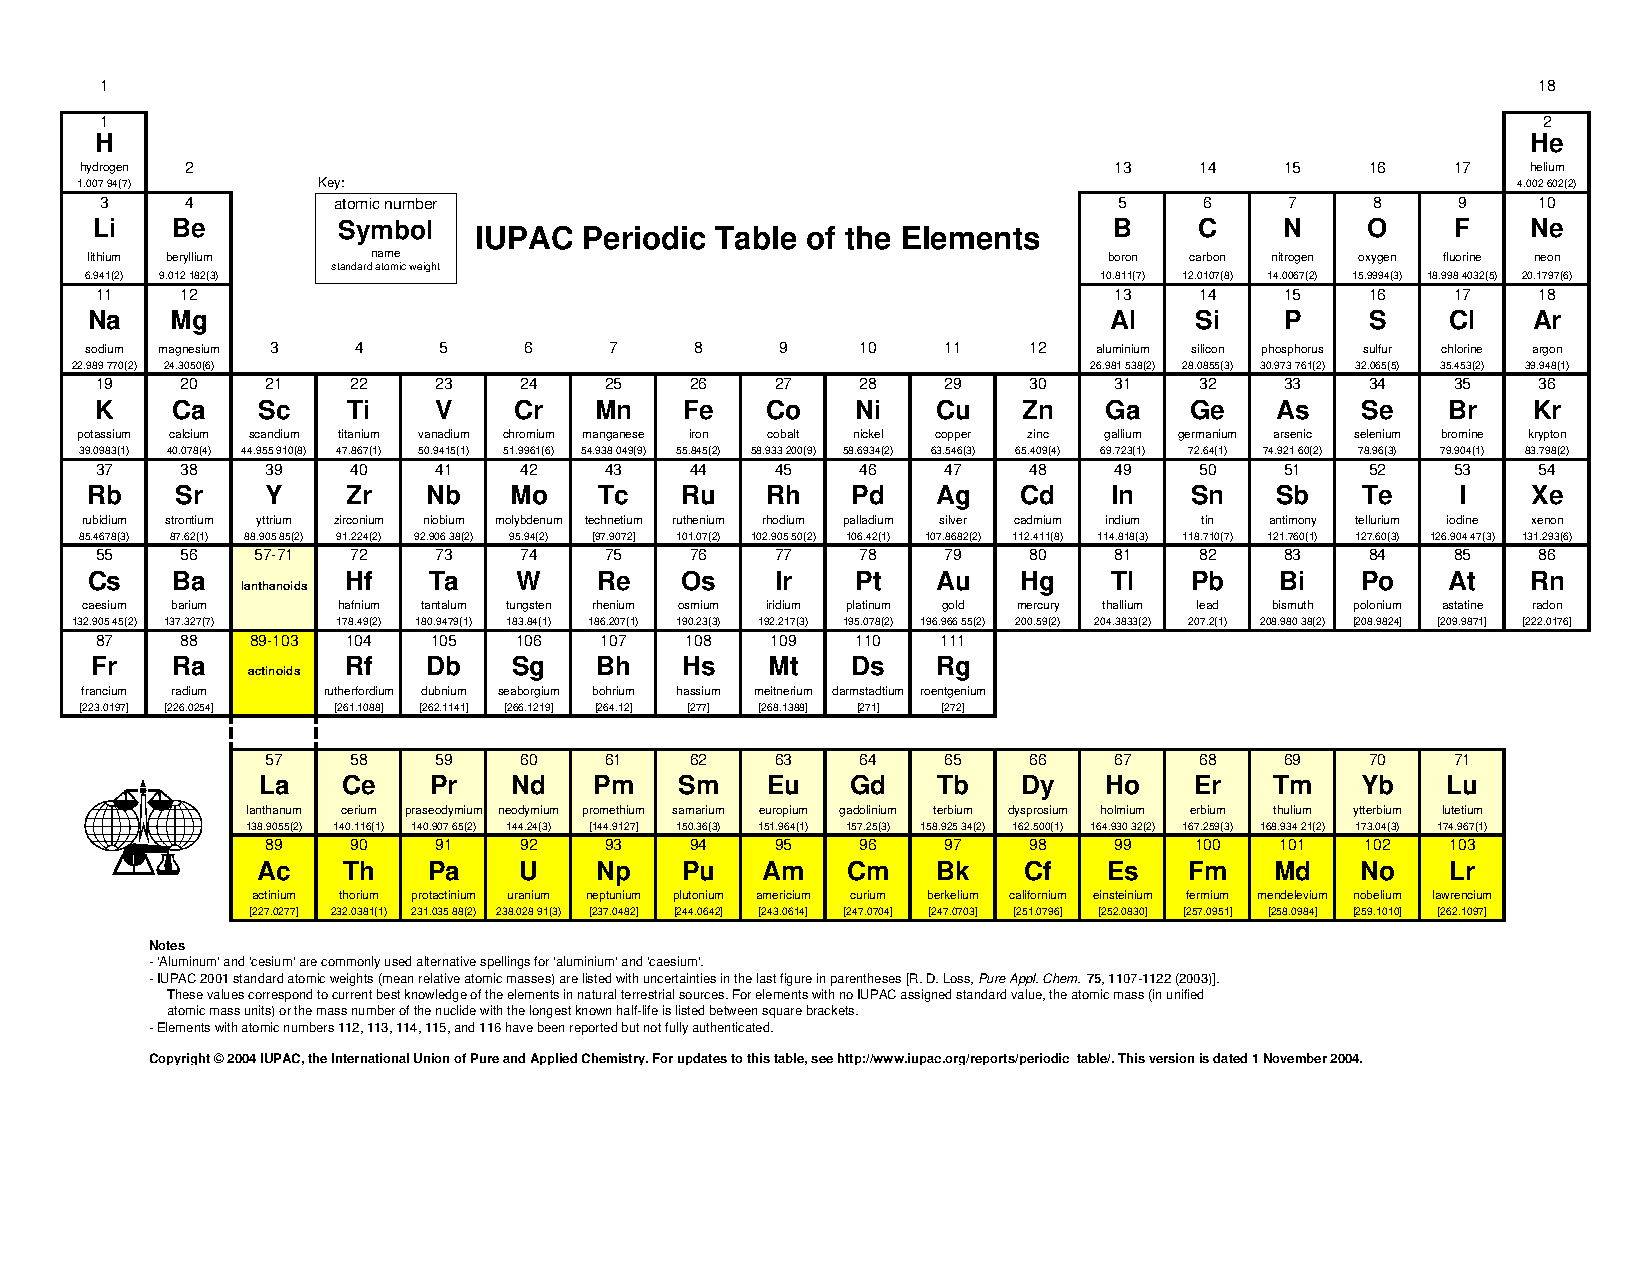
\includegraphics[width=1.00\textheight]{Appendix/PerSys.pdf}
    \end{rotate}
  \newpage
  
  \subsection{Fysische constanten}
  \label{sec:app:fysconstanten}
    \begin{tabular}{|l|c|r@{$,$}lll|}
      \hline
      \textbf{Naam} & \textbf{Symbool}  &  \multicolumn{3}{l}{\textbf{Waarde}}                   & \textbf{Eenheden}\\
      \hline
      Lading elektron        & $e$      & $1$ & $6021 $ & $ \cdot 10^{- 19}$   & $\eenh{C}$  \\ \hline
      Constante van Planck   & $h$      & $6$ & $6252 $ & $ \cdot 10^{- 34}$   & $\eenh{J}\eenh{s}$   \\ \hline
      Lichtsnelheid          & $c$      & $2$ & $99793$ & $ \cdot 10^{+ 08}$   & $\eenh{m}\eenh{s}^{-1}$ \\ \hline
      Massa van een elektron & $m_e$    & $9$ & $1083 $ & $ \cdot 10^{- 31}$   & $\eenh{kg}$  \\ \hline
      Massa van een proton   & $m_p$    & $1$ & $67239$ & $ \cdot 10^{- 27}$   & $\eenh{kg}$  \\ \hline
      Massa van een neutron  & $m_n$    & $1$ & $67470$ & $ \cdot 10^{- 27}$   & $\eenh{kg}$  \\ \hline
      Getal van Avogadro     & $N_A$    & $6$ & $0226 $ & $ \cdot 10^{+ 23}$   & $\eenh{mol}^{-1}$  \\ \hline
      Ideale gasconstante    & $R$      & $8$ & $314  $ &                      & $\eenh{J}\eenh{K}^{-1}\eenh{mol}^{-1}$ \\ 
                             &          & $0$ & $0820 $ &                      & $\eenh{l}\eenh{atm}\eenh{K}^{-1}\eenh{mol}^{-1}$ \\ 
                             &          & $1$ & $987  $ &                      & $\eenh{cal}\eenh{K}^{-1}\eenh{mol}^{-1}$ \\ \hline
      Constante van Blotzman & $\kappa$ & $1$ & $3805 $ & $ \cdot 10^{- 23}$   & $\eenh{J}\eenh{K}^{-1}$ \\ \hline
      Constante van Faraday  & $F$      & $96$ & $487 $ &                      & $\eenh{C}\eenh{mol}^{-1}$ \\ \hline
      Bohrstraal             & $a_0$    & $5$ & $2917 $ & $ \cdot 10^{- 27}$   & $\eenh{m}$  \\ \hline
      Valversnelling         & $g$      & $9$ & $81   $ &                      & $\eenh{m}\eenh{s}^{-2}$ \\ \hline
      \hline
      Correctiefactor 0001   & $\frac{RT}{F}\ln 10$       & $0$ & $0592 $ &    & \\ \hline
    \end{tabular}
  \subsection{Protolyseconstanten bij 25�C}
  \label{sec:app:protolyseconstanten}
    ..
  
  \subsection{Basiciteitsconstanten bij 25�C}
  \label{sec:app:basiciteitscontanten}
    ..
    
  \subsection{Standaardredoxpotentialen bij 25�C}
  \label{sec:app:redoxpotentialen}
    ..
    
  \subsection{Oplosbaarheidsproducten}
  \label{sec:app:oplosbaarheidsproducten}
    ..
    
  

  



   \subsection{Redoxhalfreacties opstellen}  
\label{sec:app:Halfreacties}
  \footnotesize{naar \textsc{Stefan Sandker}}
  \begin{enumerate}
    \item Begin met het redoxkoppel. 
	        Dit koppel moet bekend zijn, dus het moet expliciet in de opgave vermeld staan. 
	        Soms zul je uit de gegevens in de opgave moeten afleiden wat het koppel is, 
	        dus dan is het koppel impliciet gegeven.
	  \item \textbf{Massabalans:}
           \begin{enumerate}
	           \item Balanceer alle elementen behalve $O$ en $H$
	           \item Balanceer $O$ door het juiste aantal $H_2O$ aan te vullen.
	           \item Balanceer $H$ door het juiste aantal $H^+$ in te vullen. 
	                 Eigenlijk zou je $H_3O^+$ moet invullen, 
	                 maar in de praktijk is het gebruikelijk in redoxreacties $H^+$ in te vullen.
	         \end{enumerate}
	  \item \textbf{Ladingenbalans:}
	        Balanceer de lading door het juiste aantal $e^-$ in te vullen. 
	        Dit is overigens ook in ``gewone'' reacties belangrijk: 
	        bij het kloppend maken van een reactievergelijking moet je niet alleen de elementen kloppend maken, 
	        maar er ook altijd voor zorgen dat de lading kloppend is! In een reactievergelijking 
	        kan dat natuurlijk niet door elektronen in te vullen.
	  \item Als je bij het kloppend maken links $H^+$-ionen hebt ingevuld, maar uit de opgave blijkt dat de oplossing niet zuur is, 
	        dan moeten deze ionen verdwijnen. Dat doe je door het juiste aantal $OH^-$ toe te voegen: links ontstaat dan $H_2O$, 
	        rechts komen $OH^-$-ionen te staan. Het is ook mogelijk dat je bij het kloppend maken rechts $H^+$-ionen hebt ingevuld, 
	        terwijl uit de opgave blijkt dat dit niet correct is. Ook dan laat je de $H^+$-ionen ``verdwijnen'' door links en rechts 
	        het juiste aantal $OH^-$-ionen toe te voegen.
	  \item Controleer of tussen de deeltjes een zuur-base reactie of een neerslagreactie ontstaat.
	  \item \textbf{Vereenvoudig de halfreactie}: als je een deeltje links �n rechts ziet staan, moet je het wegstrepen.
  \end{enumerate}
   \onecolumn
\newpage
\section{Appendix: Nomenclatuur}
\label{sec:Nomenclatuur}
  \subsection{Anorganische Naamgeving}
\label{sec:HH:AnOrgNaam}
  
  \paragraph{Ionen}
  \label{sec:HHH:Ionen}
    \begin{itemize}
      \item \textbf{��natomige kationen} $X^{p+}$
	    \item \textbf{��natomige anionen} $X^{p-}$
	    \item \textbf{Enkelvoudige meeratomige anionen} $X_n^{p-}$
	    \item \textbf{Complexe anionen die zuurstof bevatten} $XO_n^{p-}$
	    \item \textbf{Complexe anionen die zuurstof en waterstof bevatten} $H_qXO_n^{q-p}$
    \end{itemize}
    
  \paragraph{Enkelvoudige stoffen $x$} 
  \label{sec:HHH:EnkelvoudigeStof}
    \begin{itemize}
      \item 
    \end{itemize}
    
  \paragraph{Binair samengestelde stoffen $x$}
  \label{sec:HHH:BinSamengestStof}
    \begin{itemize}
      \item 
    \end{itemize}
    
  \paragraph{Oxyzuren $x$ en ageleide zouten $x$}
  \label{sec:HHH:OxyzurenEnAfgZouten}
    \begin{itemize}
      \item 
    \end{itemize}
  \subsection{Organische Naamgeving}
\label{sec:HH:OrganischNaamgeving}

\begin{enumerate}
	\item De langste (hoofd)keten wordt genummerd van het ene naar het andere uiteinde met Arabische cijfers. 
	      Die nummering dient om de plaats van substituanten op de hoofdketen aan te duiden. 
	      Dit hoeft enkel te gebeuren indien de plaats van de substituant niet op ��nduidige wijze kan gedefinieerd worden.
  \item Voor de plaatsaanduiding van meerder, identieke, niet samengestelde substituanten, 
        worden passende numerieke voorvoegsels, di-, tri-, tetra-, penta-, hexa-, \ldots aangewend.
  \item De hoofdketen wordt steeds gedefinieerd als de langst mogelijk lineaire keten, 
        en op dusdanige wijze dat de substituanten dan wel de laagst mogelijke plaatsnummers toegewezen krijgen. 
        Een reeks plaatsnummers wordt als lager dan een andere beschouwd wanneer bij het eerst optredend verschil 
        tussen de twee reeksen het kleinste getal staat. 
  \item Indien twee of meerdere verschillende substituanten (zijketens) aanwezig zijn, 
        worden ze alfabetisch gerangschikt met hun respectievelijk plaatsnummer; 
        wanneer bij gelijke reeks van plaatsnummers nog steeds keuze mogelijk is, 
        wordt het laagste plaatsnummer toegewezen aan de substituant waarvan de eerste naamletter 
        ook als eerste voorkomt in het alfabet.
  \item Radicalen of substituanten afgeleid uit alkanen worden vernoemd door namen van kleinere 
        substituanten als voorvoegsel te hechten aan de naam van het langste niet vertakt radicaal 
        dat als hoofdketen fungeert. Hierbij geld zonder uitzondering dat het koolstofatoom die de 
        vrije valentie (of het ongepaard elektron) draag (of aan een andere hoofdketen gebonden wordt) 
        steeds plaatsnummer 1 toegewezen krijgt.
  \item Zoals eerder gesteld in regel 2, gebruikt men voor de aanduiding van meerdere gelijke enkelvoudige 
        substituanten de numerieke voorvoegsels di, tri, tetra, penta, hexa, \ldots. Echter, voor de aanduiding 
        van meerdere gelijke samengestelde substituanten gebruikt men de numerieke voorvoegsels bis, tris, 
        tetrakis, pentakis, hexakis \ldots
  \item Het achtervoegsel ``\textit{aan}'' wordt vervangen door
		     \begin{itemize}
		       \item ``\textit{een}''      om 1 dubbele $C=C$ binding
			     \item ``\textit{adieen}''   om	2 dubbele $C=C$ bindingen
		       \item ``\textit{atrieen}''  om 3 dubbele $C=C$ bindingen
		       \item \ldots
		     \end{itemize}
		 	  aan te duiden in de hoofdketen van een onverzadigde koolwaterstof.
  \item De hoofdketen wordt zodanig genummerd dat de dubbele bindingen de laagst mogelijke plaatsnummers 
        toegewezen krijgen. De hoofdketen is steeds deze met het hoogst aantal dubbele $C=C$-bindingen, 
        zelfs als er een andere lineaire keten met een hoger aantal $C$-atomen maar zonder dubbele 
        $C=C$-bindingen kan gevonden worden. Plaatsnummers van dubbele bindingen verwijzen naar de positie 
        van bindingen eerder dan van atomen.
  \item Het achtervoegsel ``\textit{aan}'' wordt vervangen door
          \begin{itemize}
            \item ``\textit{yn}'' 		   om	1 triple $C \equiv C$ binding					(alkyn)	
	          \item ``\textit{adiyn}''	   om 	2 triple $C\equiv C$ bindingen				(alkadiyn)
	          \item ``\textit{enyn}''	     om 	1 dubbele $C=C$ en 1 triple $C \equiv C$ binding		(alkenyn)
	          \item ``\textit{di�nyn}''	   om 	2 dubbele $C=C$ en 1 triple $C \equiv C$ bindingen		(alkadi�nyn)
	          \item ``\textit{eendiyn}''	 om	1 dubbele $C=C$ en 2 triple $C \equiv C$ bindingen		(alkeendiyn)
	          \item \ldots
	        \end{itemize}
	      aan te duiden in de hoofdketen van een onverzadigde koolwaterstof.
	\item De meervoudige bindingen krijgen de laagst mogelijk plaatsnummers in de hoofdketen, 
	      voor zover plaatsaanduiding onontbeerlijk is.
	\item Indien in eenzelfde molecule twee gelijkwaardige plaatsnummering mogelijkheden naar voren komen voor 
	      de plaatsnummering van een dubbele en een triple binding, dan wordt steeds het laagste plaatsnummer 
	      toegewezen aan de dubbele eerder dan aan de triple binding.
	\item De plaats van substituanten op aromatische ringsystemen, m.i.v. gesubstitueerde benzeenderivaten, 
	      worden aangeduid met plaatsnummers. Bij digesubstitueerde benzeenderivaten, 
	      d.w.z. benzeenringen met twee substituanten, mag men ook ortho (o), meta (m) en para (p) gebruiken 
	      om respectievelijk 1,2-, 1,3- en 1,4- substitutiepatronen aan te duiden.
	      
	      % FIGUUR
	      
	\item Koolwaterstofachtige substituanten $R$, van de gedaante $C_xH_y$, kunnen van twee�rlei aard zijn, alifatisch of aromatisch. 
	      Ze zijn aromatisch als de substitutieplaats in de substituant een koolstofatoom is van een aromatisch systeem. 
	      Zulke substituanten worden aryl groepen genoemd, en worden vaak voorgesteld als Ar. 
	      De fenyl groep, $C_6H_5$-, is een voorbeeld van aryl-groep. In alle andere gevallen zijn de $C_xH_y$ substituanten alifatisch, 
	      en gaat het om alkyl, alkenyl of alkynyl groepen, naargelang het $C$-atoom op de substitutieplaats in de substituant 
	      respectievelijk $sp^3$, $sp^2$ of $sp$ gehybridiseerd is, in welk geval ze eerder voorgesteld worden als $R$.\par
	      
	      
        Bij de substitutieve nomenclatuur worden karakteristieke functionele groepen weergegeven als voorvoegsel of achtervoegsel 
        toegevoegd aan de naam van een stamverbinding die deze groepen niet bevat.
        Bij de radicofunctionele nomenclatuur worden functionele groepen aangeduid met achtervoegsels die gehecht worden aan de naam 
        van het radicaal of de substituant die aan die functionele groep gebonden is.
  \item \textbf{substitutieve naamgeving van organische halogeniden}
        \begin{description}
	        \item[alifatisch halogenide:] $R-X$ met $X: F, Cl, Br, I$ en $R$ alkyl, alkenyl, alkynyl
	        \item[aromatisch halogenide:] $R-X$ met $X: F, Cl, Br, I$ en $R$ aryl
        \end{description}
        Een halogenide $R-X$ wordt in de substitutieve nomenclatuur vernoemd door de voorvoegsels 
        ``fluor'', ``chloor'', ``broom'', ``jood'' te plaatsen v��r de naam van de verbinding, met, indien nodig, 
        een nummer om de plaats van het halogeen op de hoofdketen aan te duiden.
  \item \textbf{radicofunctionele naamgeving van organische halogeniden}
        Radicofunctionele namen van halogeniden worden voortgebracht door de functionele klassenaam 
        ``fluoride'', ``chloride'', ``bromide'', ``jodide'' te plaatsen achter de naam van een radicaal. 
        Dit type naamgeving wordt enkel gebruikt met enkelvoudige substituanten, niet met samengestelde substitanten.
  \item \textbf{substitutieve naamgeving van alcoholen ($R-OH$)}
       \begin{description}
         \item[alcohol] $R:$ alkyl
			   \item[enol]    $R:$ alkenyl (vaak onstabiele functie)
			 \end{description}
			 De hydroxylgroep ($OH$) wordt als hoofdgroep aangeduid in de substitutieve naamgeving van alcoholen door het voorvoegsel ``ol'' 
			 te hechten aan de naam van de stamverbinding met, indien nodig, een nummer om de plaats van de hydroxylgroep op de hoofdketen aan te duiden.
 \item \textbf{meer over substitutieve naamgeving van alcoholen}\par
       Hydroxyl groepen, d.w.z. alcoholfuncties worden als substituant aangeduid met het voorvoegsel ``hydroxy'' 
       indien een andere functionele groep met voorrang voor gebruik als hoofdgroep aanwezig is, of indien een 
       hydroxyl-groep voorkomt in een zijketen.\par
       De voorrang regels bij functionele groepen zijn als volgt:
       carbonzuren > carbonzuurderivaten > ketonen > aldehyden > alcoholen > ethers > aminen > hologeniden.
 \item \textbf{radicofunctionele naamgeving van alcoholen}\par
       Radicofunctionele namen van alcoholen worden verkregen door de term ``alcohol'' te voegen aan de naam 
       van een radicaal of substituant. Ook hier wordt dit type naamgeving enkel gebruikt met 
       enkelvoudige substituanten, niet met samengestelde substituanten.
 \item \textbf{Naamgeving van fenolen ($Ar-OH$)} $Ar:$ aryl \par
       De naam van hydroxyderivaten van benzeen, fenolen dus, wordt gevormd door de uitgang ``ol'', ``diol'', \ldots te voegen 
       aan de naam van de aromatische stamverbinding. Bij aanwezigheid van andere voorrang genietende functionele groepen geldt regel 16.
 \item \textbf{substitutieve naamgeving van ethers ($R'-O-R$)} $R$, $R'$ alifatisch of aromatisch\par
       De naam van ethers, $R-O-R'$ wordt in de substitutieve naamgeving gevormd door de naam van de substituant 
       $RO$- toe te voegen aan de naam van de koolwaterstof waaruit de tweede substituant $R'$ afgeleid is. 
       De ether substituant die dienst doet als stamkoolwaterstof is doorgaans deze met de langste hoofdketen, 
       of, desgevallend, deze die een andere voorrang hebbende functionele groep bevat. 
       Is $R$- een \textit{alkyl}-groep, dan is $RO$- een \textit{akoxy}-groep.
 \item \textbf{radicofunctionele naamgeving van ethers} \par
       De naam van ethers, $R-O-R'$ wordt in de radicofunctionele naamgeving voortgebracht door 
       aan de naam van de twee substituanten $R$ en $R'$, alfabetisch gerangschikt, de term ``\textit{ether}'' toe te voegen.     
  %figuur aminen
 \item \textbf{radicofunctionele naamgeving van primaire aminen ($R-NH_2$)}\par
       De naam van primaire aminen, $R-NH_2$, worden in de radicofunctionele naamgeving voortgebracht door aan de 
       naam van de substituant, de term ``amine'' toe te voegen, met desgevallend, de nodige plaatsnummers. \par
       
       \textbf{Aminen} ($R$ alifatisch of aromatisch)
       \begin{description}
         \item[primair amine:]   $R-NH_2$
         \item[secundair amine:] $R-NH_2-R'$ en $R' \neq H$
         \item[tertiair amine:]  $R'-\stackrel{R}{N}-R''$ en $R' \neq H \neq R''$ 
       \end{description}			
       
\end{enumerate}

Regel 19 - 

		



Regel 20 - 


Aminen

			

Regel 21 - 



Regel 22 - substitutieve naamgeving van primaire aminen en polyaminen
De naam van primaire aminen of polyaminen worden in de substitutieve naamgeving voortgebracht door het achtervoegsel "amine", "diamine", "triamine",\ldots, toe te voegen aan de naam van de stamverbinding, met desgevallend, de nodige plaatsnummers. Als alternatief kan ook de naam van de stamverbinding voorafgegaan worden door het voorvoegsel "amino", "diamino", "triamino"\ldots

Regel 23 - meer over substitutieve naamgeving van primaire aminen en polyaminen
Amino groepen worden als substituant aangeduid met het voorvoegsel "amino" indien een andere functionele groep met voorrang voor gebruik als hoofdgroep aanwezig is, of indien een amino groep voorkomt in een zijketen.

Regel 24- naamgeving van secundaire en tertiaire aminen
Secundaire en tertiaire aminen worden vernoemd als N-substitutieproducten van primaire aminen. De meest complexe substituant wordt gekozen als stam dienende primaire amine.

Regel 25 - naamgeving van nitroderivaten


			nitroverbinding
			R = alifatisch of aromatisch


Nitroderivaten worden vernoemd door de nitrofunctie aan te duiden met het voorvoegsel "nitro" v��r de naam van de stamverbinding.

Regel 26 - naamgeving van aldehyden


		 	R = alifatisch of aromatisch


De naam van een aldehyde wordt gevormd door de uitgang "al" te voegen aan de naam van de koolwaterstof met hetzelfde aantal koolstofatomen die als stamverbinding dient.

Regel 27 - meer over de naamgeving van aldehyden
Indien een aldehydefunctie voorkomt als zijketen van een stamverbinding die hetzij aldehydefuncties, hetzij andere voorrang hebbende functionele groepen bevat, of die cyclisch is, wordt deze groep als substituant van de hoofdketen aangeduid met het voorvoegsel "formyl".

Regel 28 - naamgeving van ketonen


			R, R' = alifatisch of aromatisch


De naam van een keton wordt gevormd door de uitgang "on" te voegen aan de naam van de koolwaterstof met hetzelfde aantal koolstofatomen die als stamverbinding dient. Waar nodig wordt de positie van de carbonyl groep, C=O, aangeduid met een plaatsnummer. Plaatsnummers van carbonylgroepen krijgen voorrang op plaatsnummers van meervoudige bindingen.

Regel 29 - meer over naamgeving van aldehyden en ketonen
Een aldehyde of ketongroep wordt aangeduid met het voorvoegsel "oxo" indien een andere voorrang hebbende functionele groep aanwezig is.



  

   
   
   
 
 

\end{document}